% labels:
% cap:resultados
% sec:res_gridworld
% sec:res_pong
% sec:res_asteroids

% ---------------------------------------------------------------------------- %
\chapter{Resultados}
\label{cap:resultados}
% ---------------------------------------------------------------------------- %

Os resultados foram parcialmente como o esperado.
Neste capítulo, serão descritos os resultados e porque estiveram ou não dentro das expectativas.
Por conta da natureza de cada ambiente e de seus resultados, formas diferentes de avaliação foram aplicadas.

\section{\textit{Gridworld}}
\label{sec:res_gridworld}

O agente se saiu bem no \textbf{\textit{Gridworld}} conforme as expectativas, consistentemente encontrando um caminho para o objetivo com diferentes arquiteturas que não fossem drasticamente diferentes, mesmo que elas não tenham sido ótimas.
A tabela abaixo apresenta a proporção média de vezes que o agente treinado por \textit{Deep Q-Learning} e que um aleatório chegaram ao objetivo.
Para o agente treinado, o número foi obtido após ele passar por cinco treinamentos de 2000 episódios cada no mapa de tamanho 10x10 apresentado anteriormente.
O modelo final conseguiu fazer o agente chegar ao objetivo quatro vezes e exceder o número máximo de ações uma vez, pois chegou a um espaço do qual não conseguiu sair já que as melhores ações tomadas eram ir em direção às paredes adjacentes.
Para o agente aleatório, o número foi obtido após 10000 tentativas de se chegar ao objetivo, equivalente ao número de episódios que o agente treinado teve para chegar ao objetivo.

\begin{center}
\begin{tabular}{l c}
\hline
Jogador & \% de chegadas ao objetivo \\
\hline
Aleatório & 1.74\% \\
DQL & 66.15\% \\
\hline
\end{tabular}
\label{table:gridworld_score}
\end{center}

Alguns experimentos diferentes, mas menos aprofundados, com menos treinamentos indicaram que número e posicionamento de armadilhas, e tamanho da \textit{grid} têm considerável influência no modelo construído.
Por um lado, o agente encontrou caminhos até o objetivo com mais velocidade e consistência, uma vez que há menos estados a serem explorados e calculados.
Por outro, a quantidade de armadilhas e locais em que são colocadas tiveram maior impacto no aprendizado; quando há muitas armadilhas ou ficam muito próximas do objetivo, tornou-se mais comum o agente não conseguir alcançá-lo, pois ele tenta evitar as recompensas negativas a ponto de ficar preso em \textit{loops} entre alguns estados ou tentar mover-se contra uma parede.
Esses problemas poderiam ser resolvidos com a escolha de hiperparâmetros melhores.

\section{\textit{Pong}}
\label{sec:res_pong}

\textbf{\textit{Pong}} mostrou uma arquitetura bem mais sensível, com pequenas alterações nos hiperparâmetros fazendo o aprendizado se tornar muito mais lento ou sequer acontecer.
Mesmo assim, os resultados se mostraram promissores dado tempo suficiente para o agente treinar e aprender.

\begin{figure}[h!]
  \begin{minipage}[b]{.5\textwidth}
  \centering
  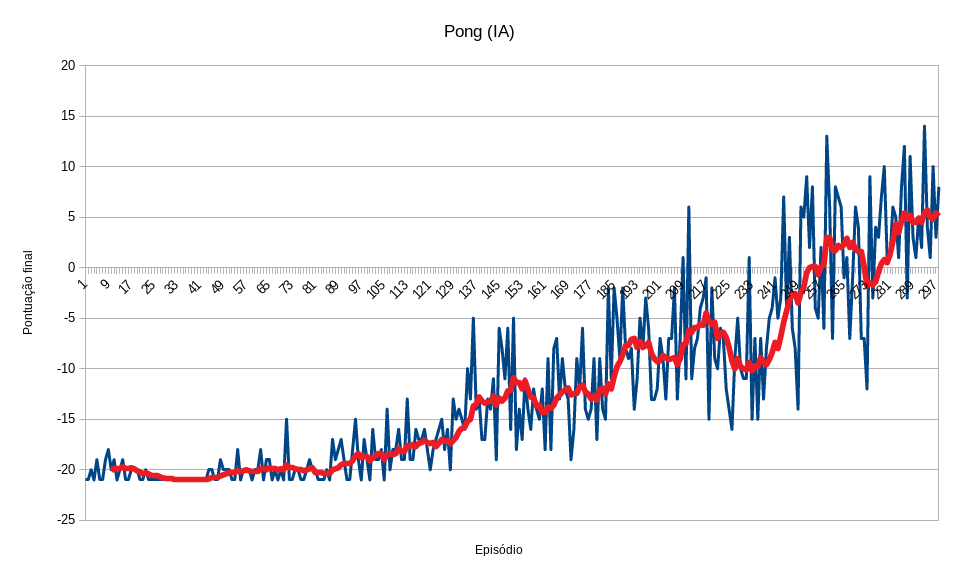
\includegraphics[scale=.3]{pong_ai_score}
  \end{minipage}
  \hfill
  \begin{minipage}[b]{.5\textwidth}
  \centering
  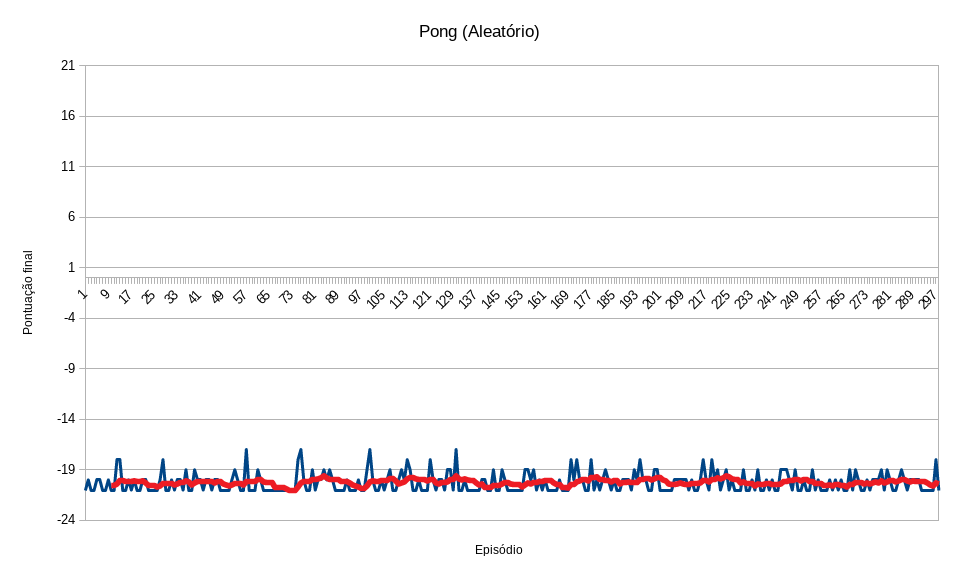
\includegraphics[scale=.3]{pong_random_score}
  \end{minipage}
  \caption{A imagem da esquerda mostra a pontuação ao longo do aprendizado e a da direita de um agente aleatório, ambos ao longo de 298 episódios, o que corresponde a aproximadamente um milhão de \textit{frames}. Cada episódio corresponde a uma partida. A linha azul é a pontuação por episódio enquanto a vermelha é a média dos últimos 10 episódios.}
  \label{fig:pong_score}
\end{figure}

O crescimento lento, mas estável da pontuação total obtida por episódio reflete a capacidade do agente de aprender, ainda que com dificuldade, a se comportar nesse ambiente de maneira positiva.

Nos experimentos, foram coletadas a pontuação final média obtida por uma pessoa experiente jogando com o mouse no emulador Stella, por um agente jogando aleatoriamente, e pela inteligência artificial treinada, cada um jogando cinco partidas contra a inteligência artificial padrão do jogo.

\begin{center}
\begin{tabular}{l c}
\hline
Jogador & Pontuação média \\
\hline
Humano & 7 \\
Aleatório & -20.27 \\
DQL & 21 \\
\hline
\end{tabular}
\label{table:pong_score}
\end{center}

\section{\textit{Asteroids}}
\label{sec:res_asteroids}
O agente não obteve resultados positivos em \textbf{\textit{Asteroids}} ao longo dos vários testes feitos.
Apesar de ser um ambiente propício para o aprendizado por \textit{Deep Q-Learning}, tendo todas as informações claras na tela, ações bem definidas e recebimento de recompensas simples e consistente, o agente teve grande dificuldade em conseguir aprender.
Por conta dessas características, esperava-se que ele conseguisse aprender a se comportar nesse domínio, ainda que com dificuldade.

Os gráficos da figura \ref{fig:asteroids_score} foram obtidos pelo agente treinado com a arquitetura de rede e treinamento descritos no capítulo \hyperref[cap:implementacao]{Implementação}, exemplificando as pontuações obtidas nos treinamentos pelos quais passou, e por um agente aleatório.

\begin{figure}[t]
  \begin{minipage}[t]{.5\textwidth}
  \centering
  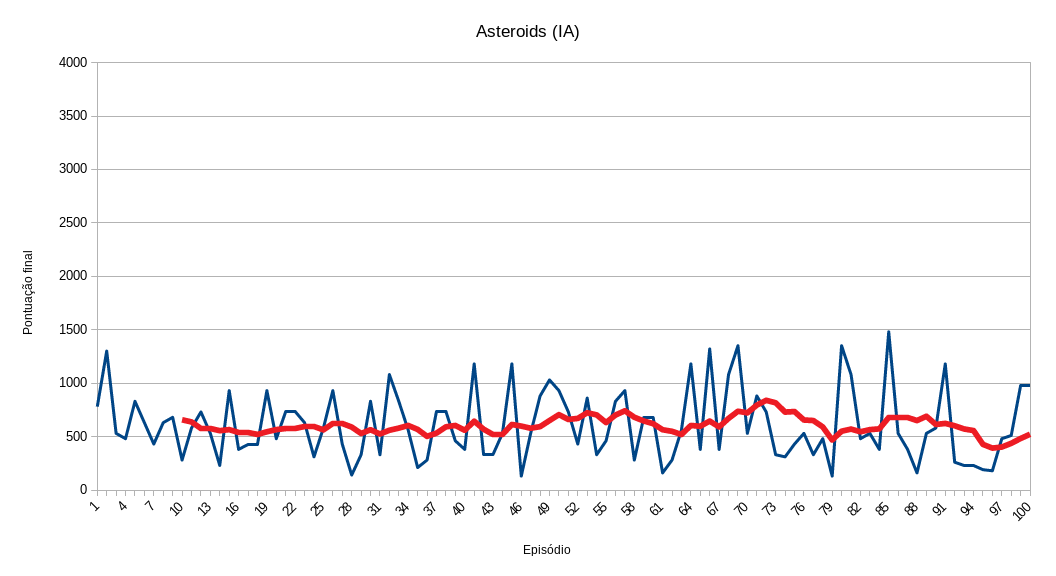
\includegraphics[scale=.3]{asteroids_ai_score}
  \end{minipage}
  \hfill
  \begin{minipage}[t]{.5\textwidth}
  \centering
  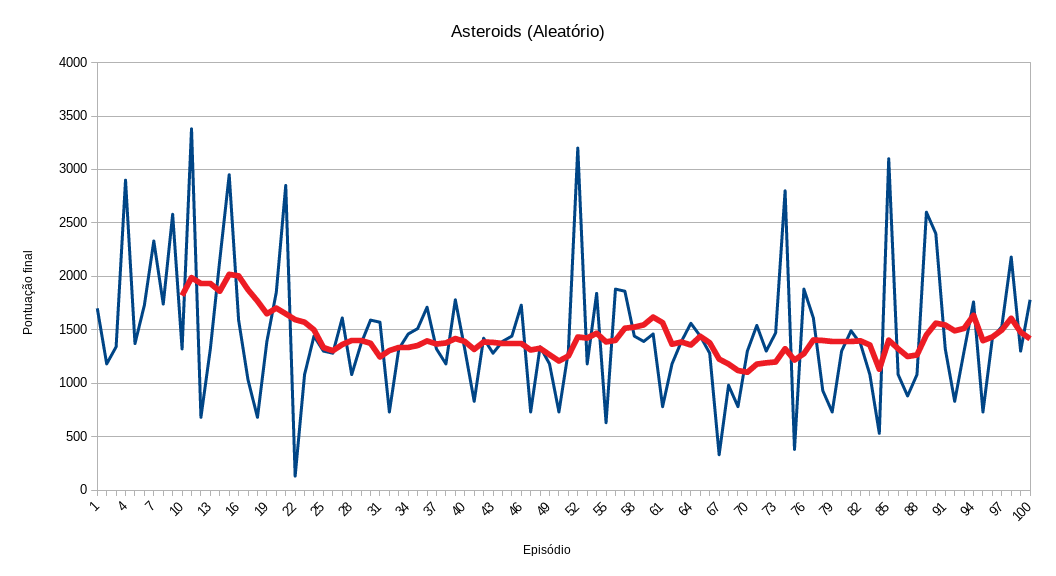
\includegraphics[scale=.3]{asteroids_random_score}
  \end{minipage}
  \caption{A imagem da esquerda mostra a pontuação ao longo do aprendizado e a da direita de um agente aleatório. A linha azul indica a pontuação final do agente nos episódios enquanto a vermelha indica a média da pontuação final dos 10 episódios anteriores.}
  \vspace*{8in}
  \label{fig:asteroids_score}
\end{figure}

Percebe-se que o agente não conseguiu aprender ou sequer mostrar indícios de melhoria mesmo com um tempo de aprendizado (em \textit{frames}) próximo do \textit{Pong}.
Nos experimentos, foram coletadas a pontuação final média de uma pessoa sem experiência, de um agente jogando aleatoriamente e da inteligência artificial treinada, cada um jogando cinco partidas.
A pontuação de jogadores experientes não foi considerada por estar muito acima, passando com facilidade dos 30000 pontos, não sendo um bom parâmetro de comparação.

\begin{center}
\begin{tabular}{l c}
\hline
Jogador & Pontuação média \\
\hline
Humano & 1943.3 \\
Aleatório & 1458.1 \\
DQL & 607.8 \\
\hline
\end{tabular}
\label{table:asteroids_score}
\end{center}

